\documentclass[a4paper]{article}    % define document layout
%\documentclass[draft]{article}     % use draft option in packages
%-----------------------------
% preamble
%-----------------------------
\usepackage[sumlimits,]{amsmath}    % math equations and formulas
\usepackage{amsfonts}
\usepackage[utf8]{inputenc}         % use UTF-8 encoding
\usepackage[english]{babel}         % use English language
\usepackage{graphicx}              % insert images
%\usepackage[draft]{graphicx}        % do not render figures
\usepackage{subcaption}             % multiple images in one figure
\usepackage{hyperref}               % hyperlinks
\usepackage{float}                  % floating objects (figures, tables)
\usepackage{geometry}               % page size and margins
\geometry{a4paper, margin=1in}      % margins
\usepackage{ragged2e}               % text alignment
\usepackage[table]{xcolor}          % change cell color in tables
%\usepackage{multirow}               % merge rows in table
%\usepackage[thinc]{esdiff}          % macros for derivatives

% MATLAB code
\usepackage{listings}
\usepackage{color} %red, green, blue, yellow, cyan, magenta, black, white
\usepackage{xcolor}

\graphicspath{                      % path for figures
    {../figures/} 
    {../figures/Q8/} 
    %{../figures/Q9/mnist/}
    %{../figures/Q9/fashion_mnist/}
    %{../figures/Q10/} 
}

\definecolor{Gray}{gray}{0.8}
\definecolor{codegreen}{rgb}{0,0.6,0}
\definecolor{codegray}{rgb}{0.5,0.5,0.5}
\definecolor{codepurple}{rgb}{0.58,0,0.82}
\definecolor{backcolour}{rgb}{0.95,0.95,0.92}

\lstdefinestyle{mystyle}{
    backgroundcolor=\color{backcolour},   
    commentstyle=\color{codegreen},
    keywordstyle=\color{magenta},
    numberstyle=\tiny\color{codegray},
    stringstyle=\color{codepurple},
    basicstyle=\ttfamily\footnotesize,
    breakatwhitespace=false,         
    breaklines=true,                 
    captionpos=b,                    
    keepspaces=true,                 
    numbers=left,                    
    numbersep=5pt,                  
    showspaces=false,                
    showstringspaces=false,
    showtabs=false,                  
    tabsize=2
}
\lstset{style=mystyle}

%-----------------------------
% body
%-----------------------------
\begin{document}

\begin{figure}
    \centering
    % UNICAMP logo
    \begin{subfigure}{0.45\textwidth}
        \centering
        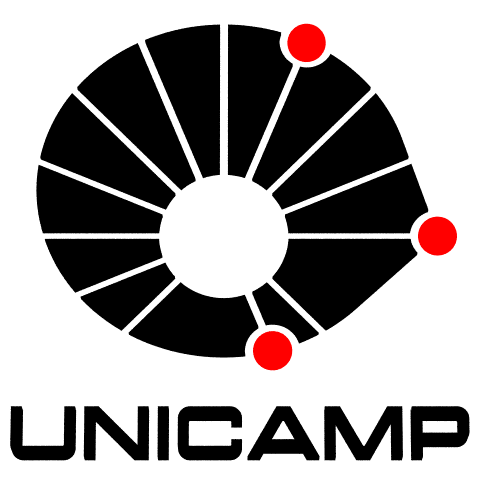
\includegraphics[width=1.5cm]{unicamp}
%        \label{fig:unicamp}
    \end{subfigure}
    \hfill
    % FEEC logo
    \begin{subfigure}{0.45\textwidth}
        \centering
        
\includegraphics[width=1.5cm]{feec}
%        \label{fig:feec}
    \end{subfigure}
\end{figure}

\title{
    \vspace{5cm}
    IA353A - Neural Networks\\
    EFC4
    \vspace{1cm}
}
\author{
    Rafael Claro Ito\\
    (R.A.: 118430)
    \vspace{11cm}
}
%R.A.: 118430
%ito.rafael@gmail.com
\date{July 2020}
\maketitle
\newpage

%=================================================
\section*{Question 8: RL}
%=================================================
\addtocounter{section}{8}

\paragraph{The Jupyter notebook related to this section with the results presented here can be opened in Google Colab environment with following link:\\}

\href{https://drive.google.com/file/d/1Xya6E4BgNVOPlzPRKbb3C59rvKI6V2nk/view?usp=sharing}{https://drive.google.com/file/d/1Xya6E4BgNVOPlzPRKbb3C59rvKI6V2nk/view?usp=sharing}

%-------------------------------------------------
\subsection{Training results and two study cases}
%-------------------------------------------------

%------------------------
\subsubsection{Maze 1}
%------------------------

\begin{figure}[H]
    \centering
    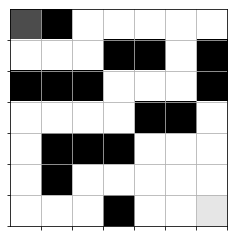
\includegraphics[width=5cm]{maze1-maze}
    \caption{Maze 1}
    \label{fig:maze1}
\end{figure}

\begin{table}[H]
    \begin{center}
        \begin{tabular}{|c|c|c|c|c|c|}
            \cline{1-6}
            \rowcolor{Gray}
            Epoch & Loss & Episodes & Win count & Win rate & Time \\
            \cline{1-6}
             0 & 0.0317 &  51 &  1 & 0.000 &   2.7 s \\
            10 & 0.0766 & 109 &  5 & 0.000 &  45.6 s \\
            20 & 0.0023 & 102 & 10 & 0.000 &  77.8 s \\
            30 & 0.0012 &   6 & 17 & 0.625 &  97.6 s \\
            40 & 0.0627 & 103 & 24 & 0.667 & 117.0 s \\
            50 & 0.0010 &   6 & 30 & 0.708 & 143.0 s \\
            60 & 0.0025 &   4 & 39 & 0.708 & 152.4 s \\
            70 & 0.0065 & 102 & 46 & 0.750 & 176.5 s \\
            80 & 0.0019 &   2 & 56 & 0.833 & 188.0 s \\
            90 & 0.0013 &  23 & 66 & 0.958 & 198.4 s \\
            94 & 0.0010 &  21 & 70 & 1.000 & 199.8 s \\
            \cline{1-6}
        \end{tabular}
    \end{center}
    \caption{Training results summary for maze 1}
    \label{tab:maze1-results}
\end{table}


%Reached 100% win rate at epoch: 94
%files: model.h5, model.json
%n_epoch: 94, max_mem: 392, data: 32, time: 200.1 seconds
%200.067352

\begin{figure}[H]
    \centering
    \begin{subfigure}{0.48\textwidth}
        \centering
        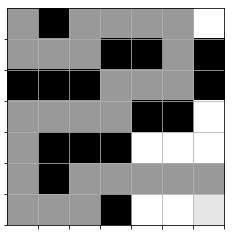
\includegraphics[width=5cm]{maze1-case1}
        \caption{Maze 1 - Study case 1}
        \label{fig:maze1-case1}
    \end{subfigure}
    \hfill
    \begin{subfigure}{0.48\textwidth}
        \centering
        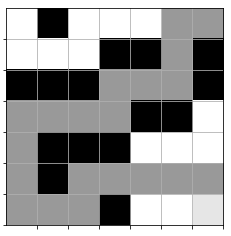
\includegraphics[width=5cm]{maze1-case2}
        \caption{Maze 1 - Study case 2}
        \label{fig:maze1-case2}
    \end{subfigure}
\end{figure}

\newpage
%------------------------
\subsubsection{Maze 2}
%------------------------

\begin{figure}[H]
    \centering
    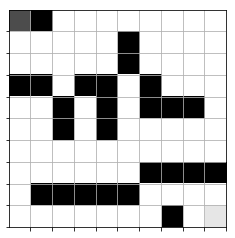
\includegraphics[width=5cm]{maze2-maze}
    \caption{Maze 2}
    \label{fig:maze2}
\end{figure}

\begin{table}[H]
    \begin{center}
        \begin{tabular}{|c|c|c|c|c|c|}
            \cline{1-6}
            \rowcolor{Gray}
            Epoch & Loss & Episodes & Win count & Win rate & Time \\
            \cline{1-6}
              0 & 0.0856 & 147 &   1 & 0.000 &   8.8 s  \\
             10 & 0.0011 & 219 &   4 & 0.000 & 128.4 s  \\
             20 & 0.0042 &  55 &   6 & 0.000 & 237.7 s  \\
             30 & 0.0041 &  21 &  13 & 0.000 & 297.6 s  \\
             40 & 0.0044 &  67 &  22 & 0.000 & 346.0 s  \\
             50 & 0.0026 &  30 &  31 & 0.600 & 380.5 s  \\
             60 & 0.0043 &  23 &  41 & 0.740 & 6.69 min \\
             70 & 0.0006 &  18 &  51 & 0.900 & 7.00 min \\
             80 & 0.0071 &  35 &  61 & 0.960 & 7.44 min \\
             90 & 0.0005 &  18 &  71 & 0.980 & 7.67 min \\
            100 & 0.0015 &   4 &  81 & 1.000 & 7.92 min \\
            110 & 0.0010 &  11 &  91 & 1.000 & 8.16 min \\
            120 & 0.0008 &  18 & 101 & 1.000 & 8.43 min \\
            130 & 0.0004 &  19 & 111 & 1.000 & 8.84 min \\
            140 & 0.0012 &  20 & 121 & 1.000 & 9.13 min \\
            150 & 0.0007 &  34 & 131 & 1.000 & 9.54 min \\
            160 & 0.0013 &  61 & 141 & 1.000 & 9.83 min \\
            165 & 0.0002 &  28 & 146 & 1.000 & 9.99 min \\
            \cline{1-6}
        \end{tabular}
    \end{center}
    \caption{Training results summary for maze 2}
    \label{tab:maze2-results}
\end{table}

%Reached 100% win rate at epoch: 165
%files: model.h5, model.json
%n_epoch: 165, max_mem: 800, data: 32, time: 10.01 minutes
%600.636667

\begin{figure}[H]
    \centering
    \begin{subfigure}{0.48\textwidth}
        \centering
        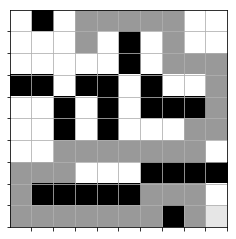
\includegraphics[width=5cm]{maze2-case1}
        \caption{Maze 2 - Study case 1}
        \label{fig:maze2-case1}
    \end{subfigure}
    \hfill
    \begin{subfigure}{0.48\textwidth}
        \centering
        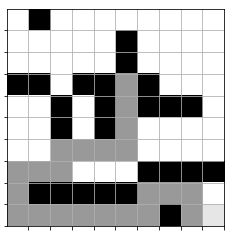
\includegraphics[width=5cm]{maze2-case2}
        \caption{Maze 2 - Study case 2}
        \label{fig:maze2-case2}
    \end{subfigure}
\end{figure}

%-------------------------------------------------
\subsection{Q-value for three different states}
%-------------------------------------------------

\subsubsection{Maze 1 - Study case 1}

\begin{figure}[H]
    \centering
    \begin{subfigure}{0.24\textwidth}
        \centering
        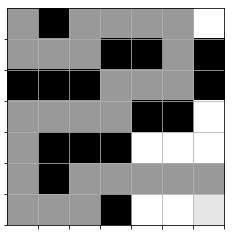
\includegraphics[width=2.8cm]{maze1-case1}
        \caption{Maze 1: Study case 1 \vspace{12mm}}
        \label{fig:maze1-case1-states}
    \end{subfigure}
    \hfill
    \centering
    \begin{subfigure}{0.24\textwidth}
        \centering
        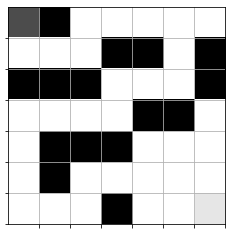
\includegraphics[width=2.8cm]{maze1-case1-state1}
        \caption{State 1 \\
            \scriptsize
            \hspace*{5mm} $\boldsymbol{\cdot}$ left:  -0.6266 \\
            \hspace*{5mm} $\boldsymbol{\cdot}$ up:    -0.4188 \\
            \hspace*{5mm} $\boldsymbol{\cdot}$ right: -0.0743 \\
            \hspace*{5mm} $\boldsymbol{\cdot}$ down:   0.0651 }
        \label{fig:maze1-case1-state1}
    \end{subfigure}
    \hfill
    \begin{subfigure}{0.24\textwidth}
        \centering
        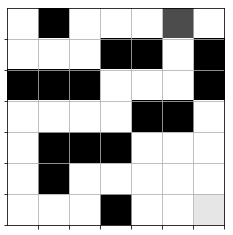
\includegraphics[width=2.8cm]{maze1-case1-state2}
        \caption{State 2 \\
            \scriptsize
            \hspace*{5mm} $\boldsymbol{\cdot}$ left:  -0.4398 \\
            \hspace*{5mm} $\boldsymbol{\cdot}$ up:    -0.4012 \\
            \hspace*{5mm} $\boldsymbol{\cdot}$ right: -0.2719 \\
            \hspace*{5mm} $\boldsymbol{\cdot}$ down:  -0.1840 }
        \label{fig:maze1-case1-state2}
    \end{subfigure}
    \hfill
    \begin{subfigure}{0.24\textwidth}
        \centering
        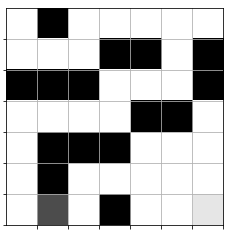
\includegraphics[width=2.8cm]{maze1-case1-state3}
        \caption{State 3 \\
            \scriptsize
            \hspace*{5mm} $\boldsymbol{\cdot}$ left: -0.0811 \\
            \hspace*{5mm} $\boldsymbol{\cdot}$ up:   -0.0670 \\
            \hspace*{5mm} $\boldsymbol{\cdot}$ right: 0.4976 \\
            \hspace*{5mm} $\boldsymbol{\cdot}$ down:  0.0538 }
        \label{fig:maze1-case1-state3}
    \end{subfigure}
\end{figure}

%------------------------
\subsubsection{Maze 1 - Study case 2}

\begin{figure}[H]
    \centering
    \begin{subfigure}{0.24\textwidth}
        \centering
        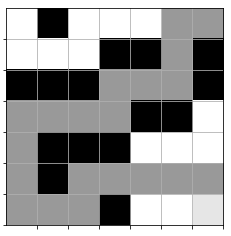
\includegraphics[width=2.8cm]{maze1-case2}
        \caption{Maze 1: Study case 2 \vspace{12mm}}
        \label{fig:maze1-case2-states}
    \end{subfigure}
    \hfill
    \centering
    \begin{subfigure}{0.24\textwidth}
        \centering
        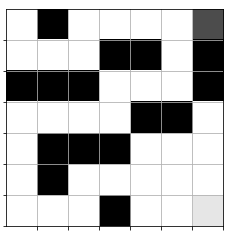
\includegraphics[width=2.8cm]{maze1-case2-state1}
        \captionsetup{singlelinecheck=off}
        \caption{State 1 \\
            \scriptsize
            \hspace*{5mm} $\boldsymbol{\cdot}$ left:  -0.3038 \\
            \hspace*{5mm} $\boldsymbol{\cdot}$ up:    -0.4816 \\
            \hspace*{5mm} $\boldsymbol{\cdot}$ right: -0.8406 \\
            \hspace*{5mm} $\boldsymbol{\cdot}$ down:  -0.4413 }
        \label{fig:maze1-case2-state1}
    \end{subfigure}
    \hfill
    \begin{subfigure}{0.24\textwidth}
        \centering
        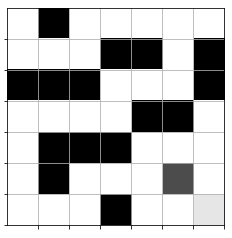
\includegraphics[width=2.8cm]{maze1-case2-state2}
        \caption{State 2 \\
            \scriptsize
            \hspace*{5mm} $\boldsymbol{\cdot}$ left:  0.3047 \\
            \hspace*{5mm} $\boldsymbol{\cdot}$ up:    0.6444 \\
            \hspace*{5mm} $\boldsymbol{\cdot}$ right: 0.9281 \\
            \hspace*{5mm} $\boldsymbol{\cdot}$ down:  0.0919 }
        \label{fig:maze1-case2-state2}
    \end{subfigure}
    \hfill
    \begin{subfigure}{0.24\textwidth}
        \centering
        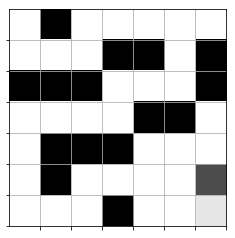
\includegraphics[width=2.8cm]{maze1-case2-state3}
        \caption{State 3 \\
            \scriptsize
            \hspace*{5mm} $\boldsymbol{\cdot}$ left:   0.3186 \\
            \hspace*{5mm} $\boldsymbol{\cdot}$ up:     0.6454 \\
            \hspace*{5mm} $\boldsymbol{\cdot}$ right: -1.9548 \\
            \hspace*{5mm} $\boldsymbol{\cdot}$ down:   1.0120 }
        \label{fig:maze1-case2-state3}
    \end{subfigure}
\end{figure}

%------------------------
\subsubsection{Maze 2 - Study case 1}

\begin{figure}[H]
    \centering
    \begin{subfigure}{0.24\textwidth}
        \centering
        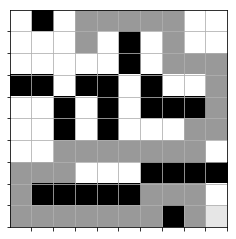
\includegraphics[width=2.8cm]{maze2-case1}
        \caption{Maze 1: Study case 1 \vspace{12mm}}
        \label{fig:maze2-case1-states}
    \end{subfigure}
    \hfill
    \centering
    \begin{subfigure}{0.24\textwidth}
        \centering
        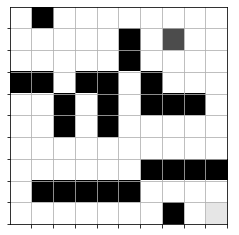
\includegraphics[width=2.8cm]{maze2-case1-state1}
        \caption{State 1 \\
            \scriptsize
            \hspace*{5mm} $\boldsymbol{\cdot}$ left:  -0.5747 \\
            \hspace*{5mm} $\boldsymbol{\cdot}$ up:    -0.4207 \\
            \hspace*{5mm} $\boldsymbol{\cdot}$ right: -0.4067 \\
            \hspace*{5mm} $\boldsymbol{\cdot}$ down:  -0.3697 }
        \label{fig:maze2-case1-state1}
    \end{subfigure}
    \hfill
    \begin{subfigure}{0.24\textwidth}
        \centering
        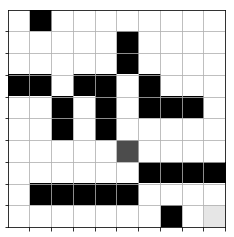
\includegraphics[width=2.8cm]{maze2-case1-state2}
        \caption{State 2 \\
            \scriptsize
            \hspace*{5mm} $\boldsymbol{\cdot}$ left:  -0.2018 \\
            \hspace*{5mm} $\boldsymbol{\cdot}$ up:    -0.6692 \\
            \hspace*{5mm} $\boldsymbol{\cdot}$ right: -0.5693 \\
            \hspace*{5mm} $\boldsymbol{\cdot}$ down:  -0.6134 }
        \label{fig:maze2-case1-state2}
    \end{subfigure}
    \hfill
    \begin{subfigure}{0.24\textwidth}
        \centering
        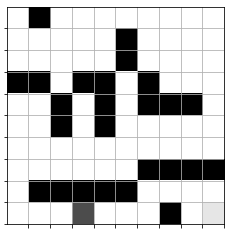
\includegraphics[width=2.8cm]{maze2-case1-state3}
        \caption{State 3 \\
            \scriptsize
            \hspace*{5mm} $\boldsymbol{\cdot}$ left:   0.1001 \\
            \hspace*{5mm} $\boldsymbol{\cdot}$ up:    -0.1958 \\
            \hspace*{5mm} $\boldsymbol{\cdot}$ right:  0.4426 \\
            \hspace*{5mm} $\boldsymbol{\cdot}$ down:  -0.0384 }
        \label{fig:maze2-case1-state3}
    \end{subfigure}
\end{figure}

%------------------------
\subsubsection{Maze 2 - Study case 2}

\begin{figure}[H]
    \centering
    \begin{subfigure}{0.24\textwidth}
        \centering
        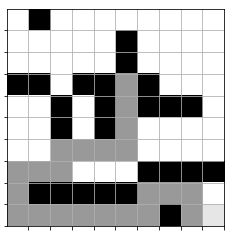
\includegraphics[width=2.8cm]{maze2-case2}
        \caption{Maze 2: Study case 2 \vspace{12mm}}
        \label{fig:maze2-case2-states}
    \end{subfigure}
    \hfill
    \centering
    \begin{subfigure}{0.24\textwidth}
        \centering
        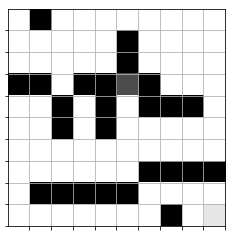
\includegraphics[width=2.8cm]{maze2-case2-state1}
        \caption{State 1 \\
            \scriptsize
            \hspace*{5mm} $\boldsymbol{\cdot}$ left:  -0.5848 \\
            \hspace*{5mm} $\boldsymbol{\cdot}$ up:    -0.6763 \\
            \hspace*{5mm} $\boldsymbol{\cdot}$ right: -0.4808 \\
            \hspace*{5mm} $\boldsymbol{\cdot}$ down:  -0.2210 }
        \label{fig:maze2-case2-state1}
    \end{subfigure}
    \hfill
    \begin{subfigure}{0.24\textwidth}
        \centering
        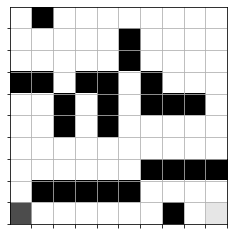
\includegraphics[width=2.8cm]{maze2-case2-state2}
        \caption{State 2 \\
            \scriptsize
            \hspace*{5mm} $\boldsymbol{\cdot}$ left:  -0.0098 \\
            \hspace*{5mm} $\boldsymbol{\cdot}$ up:    -0.2776 \\
            \hspace*{5mm} $\boldsymbol{\cdot}$ right:  0.2342 \\
            \hspace*{5mm} $\boldsymbol{\cdot}$ down:   0.0314 }
        \label{fig:maze2-case2-state2}
    \end{subfigure}
    \hfill
    \begin{subfigure}{0.24\textwidth}
        \centering
        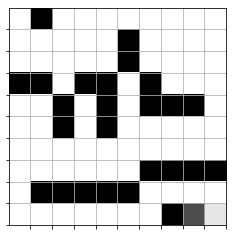
\includegraphics[width=2.8cm]{maze2-case2-state3}
        \caption{State 3 \\
            \scriptsize
            \hspace*{5mm} $\boldsymbol{\cdot}$ left:  -0.2766 \\
            \hspace*{5mm} $\boldsymbol{\cdot}$ up:     0.0523 \\
            \hspace*{5mm} $\boldsymbol{\cdot}$ right:  0.9958 \\
            \hspace*{5mm} $\boldsymbol{\cdot}$ down:  -0.1527 }
        \label{fig:maze2-case2-state3}
    \end{subfigure}
\end{figure}

\newpage
%-------------------------------------------------
\subsection{RMS during the training}
%-------------------------------------------------

\paragraph{Explique como é definida a função de erro quadrático médio usada no treinamento.}

\paragraph{Inicialmente, devemos relembrar a equação de Bellman. Queremos achar a função Q-valor ótima, $Q^*$, que satisfaça a seguinte equação:}

\begin{align*}
    Q^*(s,a) = \mathbb{E}_{s'\sim \mathcal{E}}\left[r+\gamma\max_{a'}Q^*(s',a')|s,a\right]
\end{align*} 

\paragraph{A política ótima $\pi^*$ é dada se tomarmos a melhor ação de acordo com os valores da função $Q^*$.}

\paragraph{Para resolver a equação anterior, temos um algoritmo iterativo dado por:}

\begin{align*}
    Q_{i+1}(s,a) = \mathbb{E}_{s'\sim \mathcal{E}}\left[r+\gamma\max_{a'}Q^*(s',a')|s,a\right]
\end{align*} 

\paragraph{Quando $i$ tende a infinito, temos que $Q_i$ tende a $Q^*$.}
\paragraph{Entretanto, essa abordagem não é escalável. Assim o que se faz é usar uma rede neural para aprender e estimar a função Q-valor, sintetizando portanto, um mapeamento entre os estados e os q-valores.}

\paragraph{Faremos então:}
\begin{align*}
    Q(s,a;\theta) \approx Q^*(s,a)
\end{align*} 

\paragraph{Onde $\theta$ representa os parâmetros do modelo (pesos da rede neural).}

\paragraph{Assim, tomando $y_i$ como a saída da rede neural e $L_i(\theta_i)$ a função de perda usada durante seu treinamento, podemos retomar a equação de Bellman aproximando o lado direito com o lado esquerdo:}

\begin{align*}
    y_i = \mathbb{E}_{s'\sim \mathcal{E}}\left[r+\gamma\max_{a'}Q^*(s',a';\theta_{i-1})|s,a\right]
\end{align*} 
\begin{align*}
    L_i(\theta_i) = \mathbb{E}_{s,a\sim\rho}\left[(y_i - Q(s,a;\theta_i))^2\right]
\end{align*} 

\paragraph{E é justamente assim que é definida a função de erro quadrático médio usado no treinamento. Procura-se um mapeamento entre os estados, usado como entrada da rede neural (neste caso é o panorama do labirinto), e a a função Q-valor ótima. Ao minizarmos o erro quadrático médio entre a saída da rede e função Q-valor parametrizada por theta, estamos na verdade forçando que o lado esquerdo da equação de Bellman seja igual ao lado direito. Conforme o agente se movimenta e explora o ambiente, atua-se no vetor de pesos através de técnicas de gradiente, e com isso chegamos em um mapeamento onde a saída da rede neural representa a função Q-valor ótima aproximada.}

\paragraph{Para finalizar, usando como gancho para a resposta do próximo item, temos que a entrada da rede (inputs) o estado do ambiente e a saída da rede (targets) calculada como a recompensa dada pela ação tomada anteriormente mais o fator de desconto (gamma) multiplicado pelo máximo de $Q(s',a')$ (que representa o máximo da saída do próximo estado, ou apenas a recompensa em caso de game over).}

\newpage
%-------------------------------------------------
\subsection{Experience replay}
%-------------------------------------------------

\paragraph{Explique como é trabalhada a técnica de experience replay.}

\paragraph{Para se trabalhar com a técnica de experience replay, é proposta uma classe denominada Experience. Nesta classe temos o ``construtor" da classe \_\_init\_\_ (magic method, ou ainda ``dunder``) e três métodos: remember, predict e get\_data.}

\paragraph{A principal ideia aqui é usar uma memória para armazenar episódios. Um episódio é composto de uma lista com cinco elementos:}
\begin{itemize}
    \item envstate: estado do ambiente contendo os valores de todas células do labirinto (em um array 1D).
    \item action: uma das quatro ações que o agente (rato) pode tomar (cima, baixo, direita ou esquerda).
    \item reward: recompensa recebida pela ação tomada.
    \item envstate\_next: novo estado do ambiente após a ação do agente.
    \item game\_over: valor booleano que indica se houve game over (win ou lose).
\end{itemize}

\paragraph{Assim, para cada movimento do rato, temos um episódio que podemos inserir em uma memória. Conforme essa memória vai se enchendo, defini-se um limite para deletar episódios mais antigos armazenados. Neste caso em específico, adotou-se uma memória de tamanho padrão 1000, mas definindo-a como 8 vezes o tamanho do labirinto na chamada do treinamento da rede neural.}

\paragraph{O método remember é chamado após cada movimento do agente, sendo sua função armazenar as informações daquele episódio na memória. O método get\_data é usado para pegar da memória a entrada (inputs) e saída (targets) que será usado no treinamento da rede neural, sendo que o número de amostras retornado por get\_data é definido como o mínimo entre o tamanho da memória e 50 (data\_size). E é esse processo que caracteriza a técnica experience replay, armazenando experiências recentes do agente (com a premissa de quanto mais ele se movimenta no ambiente, melhor vai ficando a predição da rede neural e portanto seus próximos movimentos) e usando dessas experiências para o treinamento, dado que a solução do problema trata-se de um processo iterativo.}

\paragraph{Inicialmente, a saída da rede neural produzirá resultados aleatórios, mas conforme o treinamento for avançando e os parâmetros ajustados adequadamente, sua saída vai convergindo para a solução da equação de Bellman.}


\newpage
%=================================================
\section{Question 9: GAN}
%=================================================

\paragraph{The Jupyter notebook related to this section with the results presented here can be opened in Google Colab environment with following link:\\}

\href{https://drive.google.com/file/d/1WWdc3M0UObMp1jVCcndmor6BTdLe18\_e/view?usp=sharing}{https://drive.google.com/file/d/1WWdc3M0UObMp1jVCcndmor6BTdLe18\_e/view?usp=sharing}

%------------------------
\subsection{MNIST}
%------------------------

\graphicspath{{../figures/Q9/mnist/}}

\begin{figure}[H]
    \centering
    % epoch 0
    \begin{subfigure}{0.32\textwidth}
        \centering
        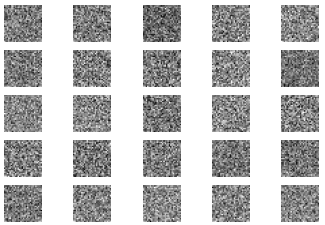
\includegraphics[width=5cm]{0}
        \caption{First image}
        \label{fig:mnist-epoch0}
    \end{subfigure}
    \hfill
    % epoch 1,000
    \begin{subfigure}{0.32\textwidth}
        \centering
        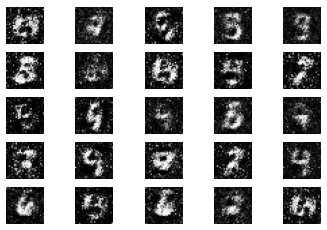
\includegraphics[width=5cm]{1000}
        \caption{After 1,000 epochs}
        \label{fig:mnist-epoch1000}
    \end{subfigure}
    \hfill
    % epoch 10,000
    \begin{subfigure}{0.32\textwidth}
        \centering
        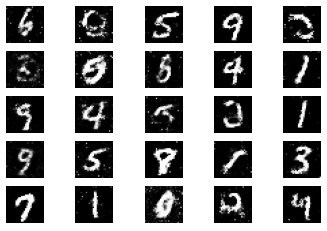
\includegraphics[width=5cm]{10000}
        \caption{After 10,000 epochs}
        \label{fig:mnist-epoch10000}
    \end{subfigure}
    \hfill
    % epoch 20,000
    \begin{subfigure}{0.32\textwidth}
        \centering
        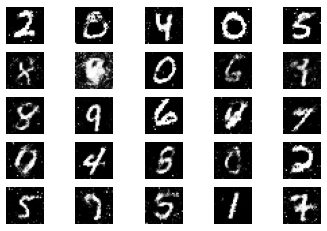
\includegraphics[width=5cm]{20000}
        \caption{After 20,000 epochs}
        \label{fig:mnist-epoch20000}
    \end{subfigure}
    \hfill
    % epoch 30,000
    \begin{subfigure}{0.32\textwidth}
        \centering
        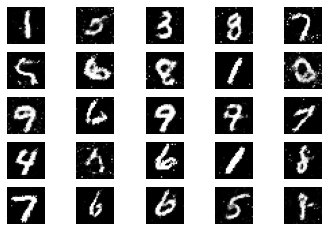
\includegraphics[width=5cm]{30000}
        \caption{After 30,000 epochs}
        \label{fig:mnist-epoch30000}
    \end{subfigure}
    \hfill
    % epoch 50,000
    \begin{subfigure}{0.32\textwidth}
        \centering
        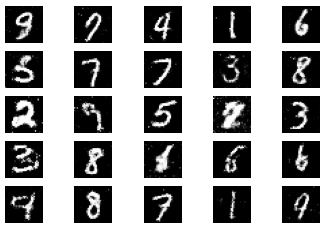
\includegraphics[width=5cm]{50000}
        \caption{After 50,000 epochs}
        \label{fig:mnist-epoch50000}
    \end{subfigure}
    % caption and label
    \caption{GAN trained for MNIST dataset} 
    \label{fig:gan-mnist}
\end{figure}


%------------------------
\subsection{Fashion MNIST}
%------------------------

\graphicspath{{../figures/Q9/fashion_mnist/}}

\begin{figure}[H]
    \centering
    % epoch 0
    \begin{subfigure}{0.32\textwidth}
        \centering
        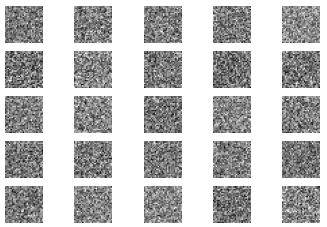
\includegraphics[width=5cm]{0}
        \caption{First image}
        \label{fig:fashion_mnist-epoch0}
    \end{subfigure}
    \hfill
    % epoch 1,000
    \begin{subfigure}{0.32\textwidth}
        \centering
        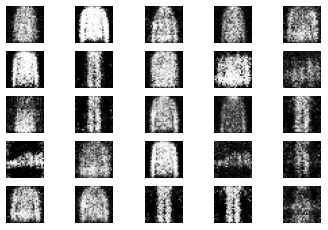
\includegraphics[width=5cm]{1000}
        \caption{After 1,000 epochs}
        \label{fig:fashion_mnist-epoch1000}
    \end{subfigure}
    \hfill
    % epoch 10,000
    \begin{subfigure}{0.32\textwidth}
        \centering
        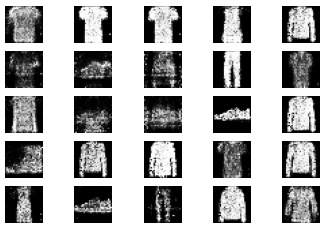
\includegraphics[width=5cm]{10000}
        \caption{After 10,000 epochs}
        \label{fig:fashion_mnist-epoch10000}
    \end{subfigure}
    \hfill
    % epoch 20,000
    \begin{subfigure}{0.32\textwidth}
        \centering
        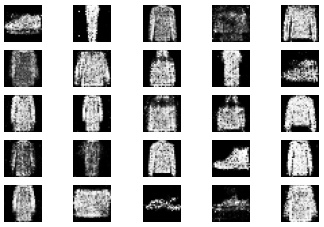
\includegraphics[width=5cm]{20000}
        \caption{After 20,000 epochs}
        \label{fig:fashion_mnist-epoch20000}
    \end{subfigure}
    \hfill
    % epoch 30,000
    \begin{subfigure}{0.32\textwidth}
        \centering
        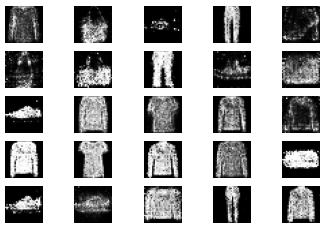
\includegraphics[width=5cm]{30000}
        \caption{After 30,000 epochs}
        \label{fig:fashion_mnist-epoch30000}
    \end{subfigure}
    \hfill
    % epoch 50,000
    \begin{subfigure}{0.32\textwidth}
        \centering
        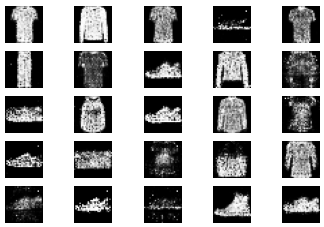
\includegraphics[width=5cm]{50000}
        \caption{After 50,000 epochs}
        \label{fig:fashion_mnist-epoch50000}
    \end{subfigure}
    % caption and label
    \caption{GAN trained for fashion MNIST dataset} 
    \label{fig:gan-fashion_mnist}
\end{figure}

\newpage
%=================================================
\section{Question 10: NLP}
%=================================================

\paragraph{The Jupyter notebook related to this section with the results presented here can be opened in Google Colab environment with following link:\\}

\href{https://drive.google.com/file/d/1EAU2toNRn-MjXyO_YAsZFejdaJDapibX/view?usp=sharing}{https://drive.google.com/file/d/1EAU2toNRn-MjXyO\_YAsZFejdaJDapibX/view?usp=sharing}

%------------------------
\subsection{Word2Vec}
%------------------------



%------------------------
\subsection{t-SNE}
%------------------------

\graphicspath{{../figures/Q10/}}

\begin{figure}[H]
    \centering
    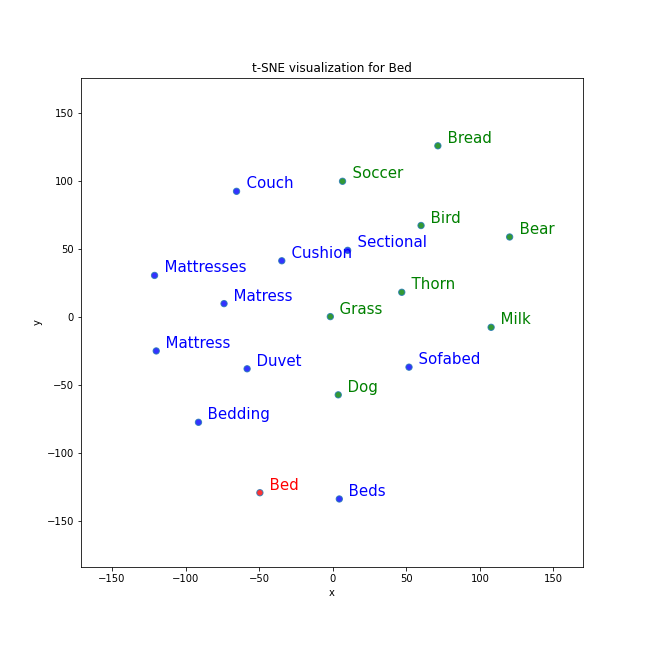
\includegraphics[width=10cm]{tsne1}
    \caption{T-SNE 1}
    \label{fig:tsne1}
\end{figure}

\begin{figure}[H]
    \centering
    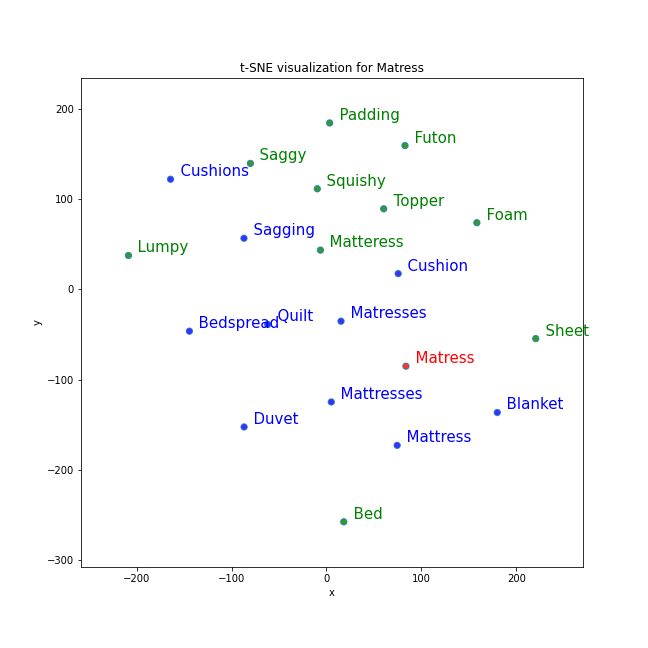
\includegraphics[width=10cm]{tsne2}
    \caption{T-SNE 2}
    \label{fig:tsne2}
\end{figure}

%------------------------
\subsection{Results discussion}
%------------------------

%=================================================

\end{document}
